\chapter{Opis projektnog zadatka}
		
	
		
		\normalsize{Papirni.ca je aplikacija koja služi za poslovanje prodavaonice papira unutar čije ponude postoje razne vrste i veličine papira uz pojedine dodatne usluge. Usluge variraju ovisno o vrsti korisnika koji se njima služi, a podjela korisnika je sljedeća: }
		
		\begin{packed_enum}
			\item  \textbf{neregistrirani korisnik}
			\item  \textbf{registrirani korisnik}
			
			\begin{packed_enum}
				
				\item privatni
				\item poslovni
				
			\end{packed_enum}
			\item  \textbf{administrator}
			
			
		\end{packed_enum}
	
		\noindent \normalsize{Neregistrirani korisnici mogu mijenjati kontekst platforme iz privatnog u poslovni i obrnuto te im je dostupno isključivo pregledavanje usluga unutar istih, dok je za kupovinu papira i/ili pružanje usluga potrebna registracija.} \\
		
		\noindent \normalsize{Registrirani privatni korisnici za prijavu koriste ime, prezime i e-mail adresu. Jedina usluga koja se pruža ovim korisnicima jest prodaja raznih vrsta papira s obzirom na sljedeće faktore: }
		
		\begin{packed_enum}
			\item \normalsize{boja}
			\item  \normalsize{vrsta}
			\item  \normalsize{težina (gsm)}
			\item  \normalsize{format (A0 - A10)}
		\end{packed_enum}
	
		\noindent \normalsize{Registrirani poslovni korisnici za prijavu koriste ime i OIB firme, ime kontakt osobe iz firme te kontaktni broj telefona i e-mail adresu iste. Kao i privatnima, poslovnim korisnicima omogućena je prodaja papira koja, uz već navedene, ima dvije dodatne opcije - izbor nekonvencionalne veličine papira po narudžbi i mogućnost dodatka vodenog žiga na papire. Korisnik mora priložiti sliku koju želi upotrijebiti kao vodeni žig ako odabere tu opciju. Osim prodaje papira, poslovnim korisnicima je omogućeno slanje posebnog tekstualnog zahtjeva putem kojeg se može zatražiti usluga koja nije u standardnoj ponudi papirnice - npr. specifičan način pakiranja narudžbe. Da bi dodatni zahtjev bio validan, korisnik mora unijeti kratki naziv usluge koju traži i kontakt podatke. Uz jednokratno korištenje usluga, poslovni korisnici mogu napraviti mjesečnu pretplatu na neki proizvod - time se odabrana kupovina obavlja automatski svaki mjesec. Ako korisnik u košarici ima proizvode koje kupuje jednokratno uz one koji su označeni za pretplatu, nakon potvrde kupnje svi će proizvodi biti naplaćeni s time da će se oni označeni za pretplatu naplaćivati mjesečno od tog trenutka do otkazivanja pretplate. Poslovni korisnik može pregledavati svoje pretplate i otkazati ih u bilo kojem trenutku.} \\
		
		\noindent \normalsize{Administratorima je omogućeno sljedeće: } 
		\begin{packed_enum}
			\item \normalsize{pregled povijesti kupljenih usluga za sve korisnike}
			\item  \normalsize{pregled i otkazivanje pretplata poslovnih korisnika}
			\item  \normalsize{pregled i mogućnost uklanjanja dodatnih uskuga dodanih putem tekstualnog zahtjeva} \\
		\end{packed_enum}
	
		\noindent \normalsize{Kupovina funkcionira na sljedeći način: odabirom na proizvod on se dodaje u košaricu, a plaćanje se vrši putem servisa PayPal. Dodatna usluga slanja tekstualnog zahtjeva se ne dodaje u košaricu nego se za nju napisani zahtjev najprije mora odobriti i tek kada (i ako) je on odobren zahtjev će se dodati tom poslovnom korisniku. U slučaju problema sa zahtjevom, korisnika se obavještava putem kontakt podataka koji su uneseni prilikom predaje zahtjeva te se istim putem i rješavaju. Nakon rješavanja potencijalnih problema dodatna usluga se dodaje korisniku, a njega se obavještava o uspješnom dodavanju usluge (također putem prethodno navedenih kontakt podataka). Takva usluga vidljiva je isključivo tom korisniku (među ostalim uslugama). } \\
		
		
		\noindent \normalsize{Projekt kao što je Papirni.ca  može koristiti bilo kojem manjem obrtu koji se bavi ovakvom djelatnošću, a uz proširenje bi se ovakva aplikacija mogla koristiti i za veće trgovine. Budući da se zbog pandemije koronavirusa naglašava smanjenje međuljudskog kontakta na minimum, online trgovine postaju sve prometnije tako da bi ovakvo rješenje bilo iznimno prikladno za papirnice koje posluju u ovo doba. Izuzevši trenutnu situaciju, ovakav pristup pogodan je udaljenim kupcima koji nisu u mogućnosti fizički posjetiti trgovinu i osobno napraviti narudžbu. Također, kupovina putem aplikacije ima određenu preglednost s izlistanim opcijama  koju kupci možda ne bi dobili jednim pogledom u fizičkoj papirnici.} 
		
		\noindent \normalsize{Primjer sličan ovome projektu je web-stranica  knjižare i papirnice Denova (\url{https://www.denova.hr/}). Njihova ponuda nije ograničena samo na papire, no kao i kod Papirni.ca aplikacije, među papirima također postoji mnogo opcija i dosta širok izbor.} \\
		
	
		%\noindent \underbar{podcrtani tekst}, \textbf{podebljani tekst}, 	%\textit{nagnuti tekst}\\
		%\noindent \normalsize primjer \large primjer \Large primjer \LARGE %{primjer} \huge {primjer} \Huge primjer \normalsize
	
		%\noindent primjer url-a: %\url{https://www.fer.unizg.hr/predmet/proinz/projekt}
		
		%\noindent posebni znakovi: \# \$ \% \& \{ \} \_ 
	%	$|$ $<$ $>$ 
	%	\^{} 
	%	\~{} 
	%	$\backslash$ 
		 %
		 %\begin{packed_item}
		 	%\item \textit{tocka}
		 	
		 %\end{packed_item}
	
		%unos slike
		\begin{figure}[H]
			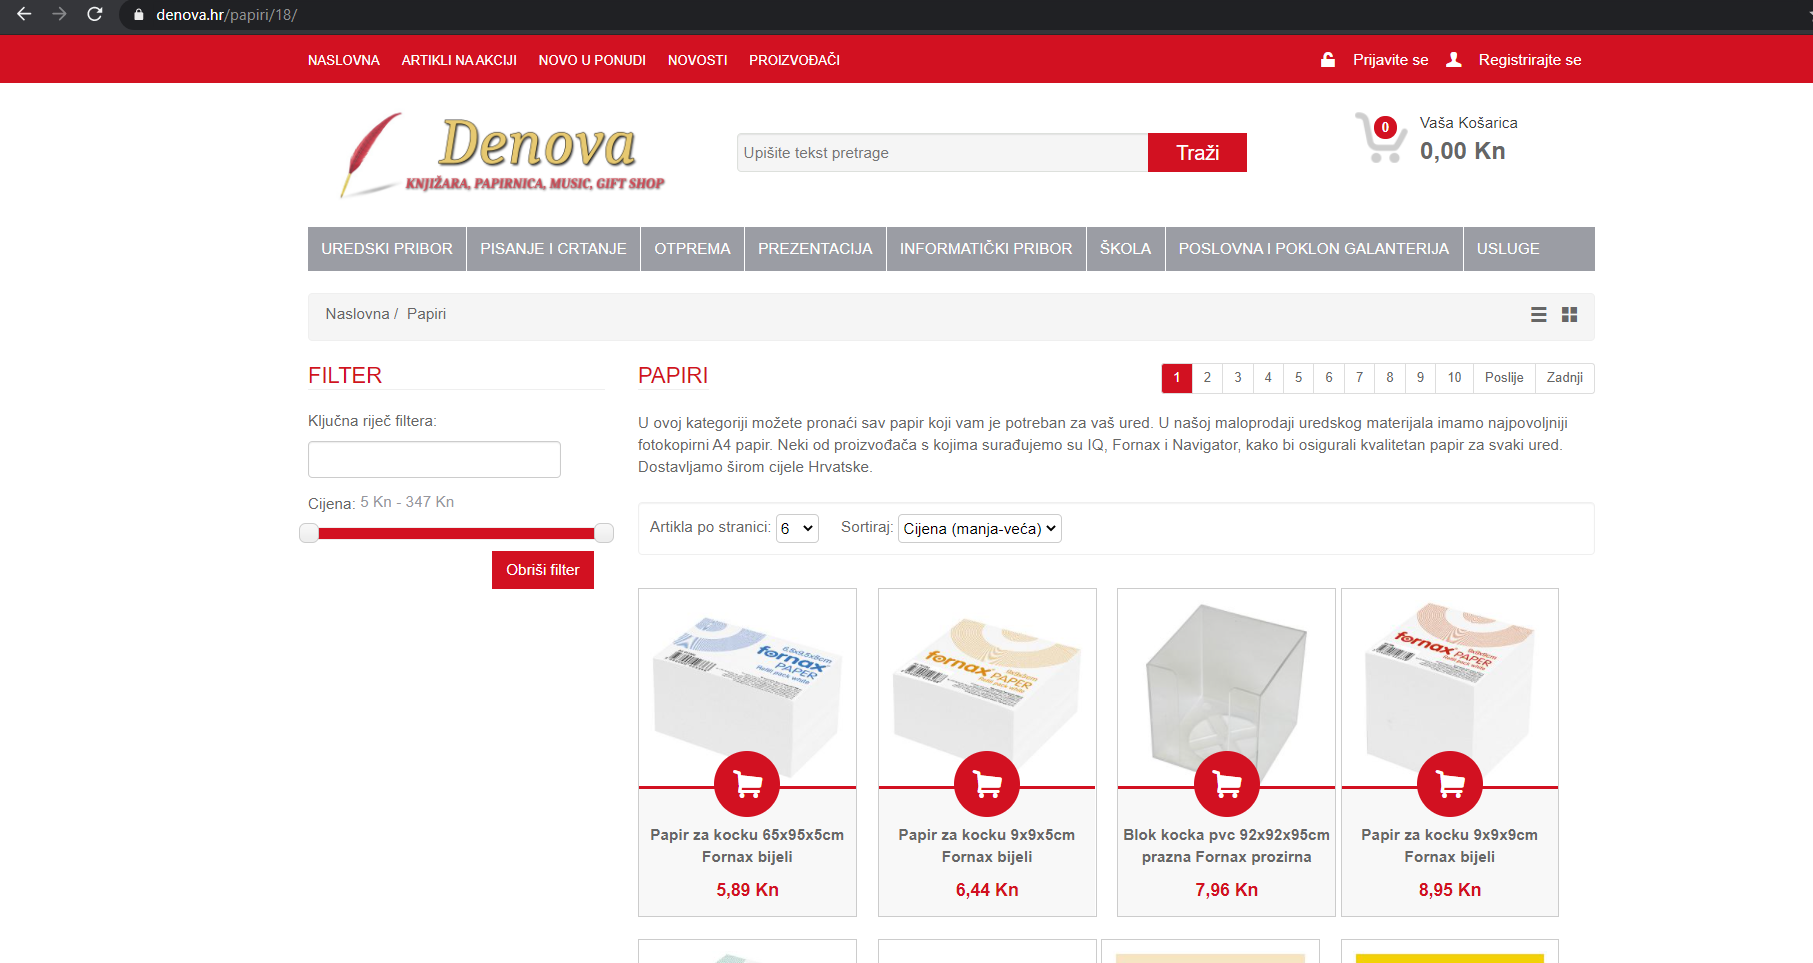
\includegraphics[scale=0.3]{slike/denova1.PNG} %veličina slike u odnosu na originalnu datoteku i pozicija slike
			
			%	\includegraphics[width=.9\linewidth]{slike/aktivnost.PNG} %veličina u odnosu na širinu linije
			\centering
			\caption{Snimka web-stranice papirnice Denova}
			\label{fig:denova1}%label mora biti drugaciji za svaku sliku
		\end{figure}
			%Referenciranje slike \ref{fig:denova1} u tekstu.
		\noindent \normalsize{   } \\
		\begin{figure}[H]
			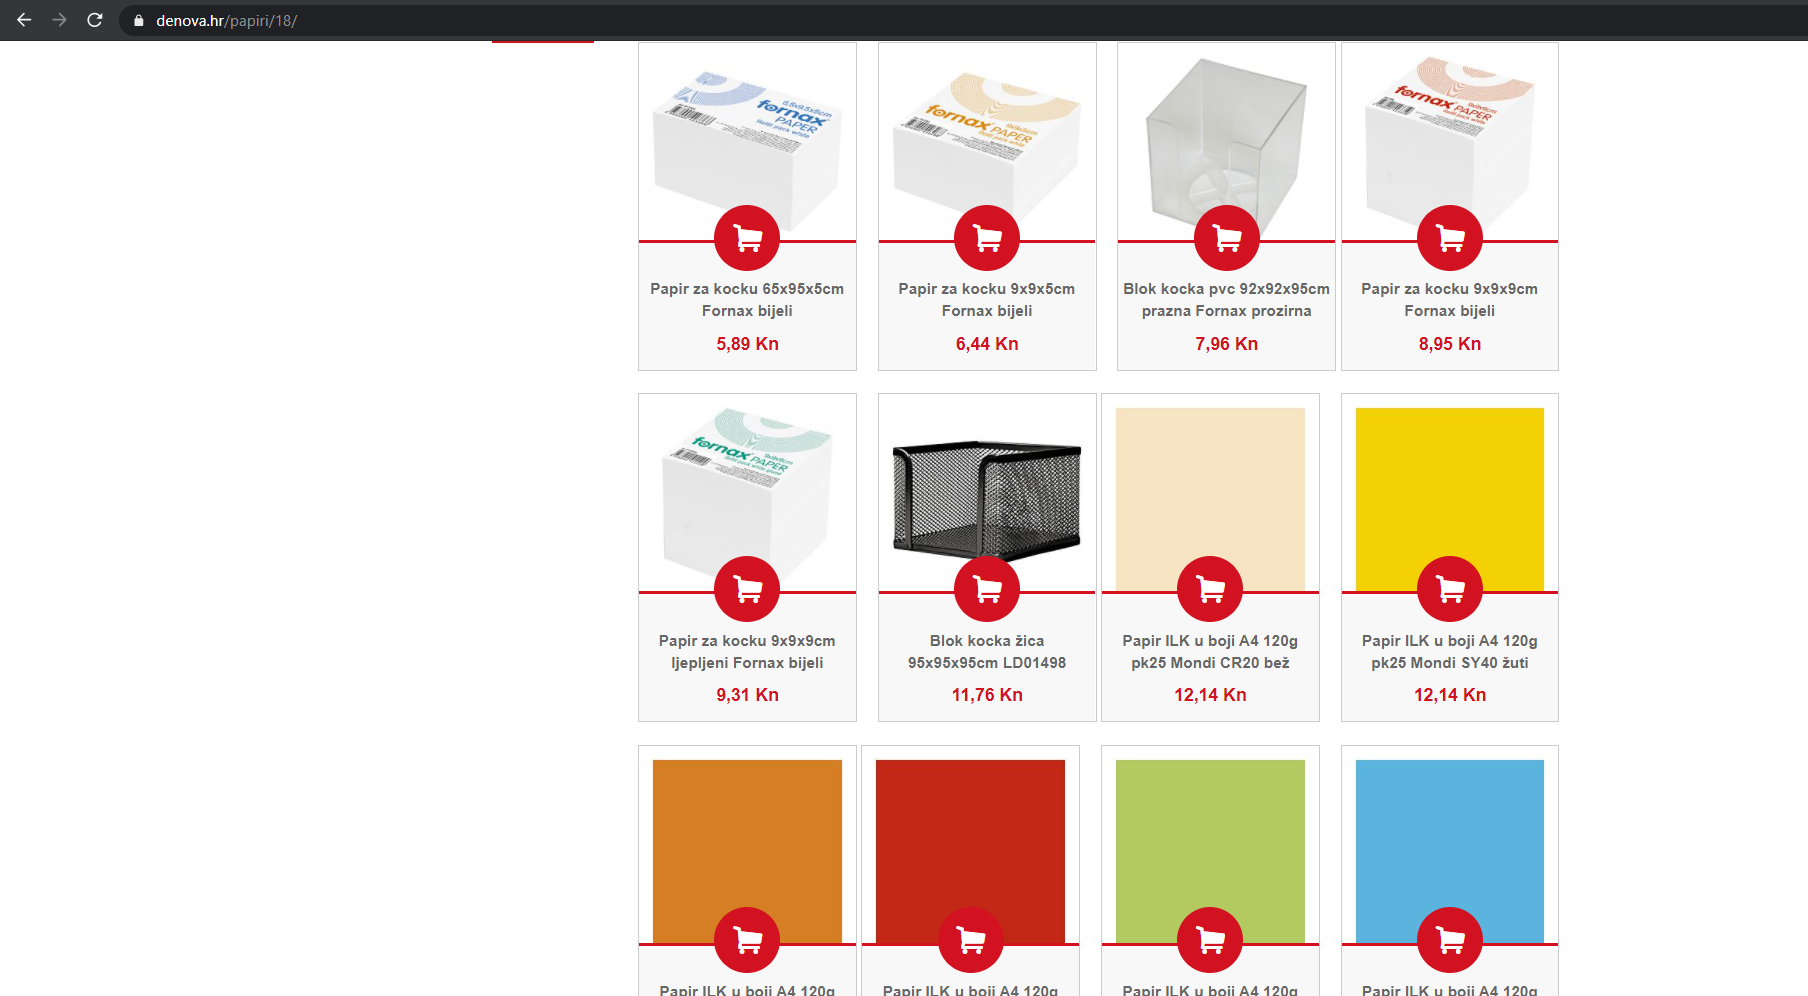
\includegraphics[scale=0.3]{slike/denova2.PNG} %veličina slike u odnosu na originalnu datoteku i pozicija slike
			
			%	\includegraphics[width=.9\linewidth]{slike/aktivnost.PNG} %veličina u odnosu na širinu linije
			\centering
			\caption{Snimka raznolike ponude papira papirnice Denova} 
			\label{fig:denova2}%label mora biti drugaciji za svaku sliku
		\end{figure}
		
		\noindent \normalsize{Papirni.ca namijenjena je svakome tko ima interes kupovati papir putem aplikacije. Za pretpostaviti je da bi se njome među privatnim korisnicima našlo dosta studenata i učenika budući da su mladi skloniji ovakvoj vrsti kupovine jer su tehnički pismeniji od starijih generacija. Dodatne usluge koje se pružaju poslovnim korisnicima zasigurno bi bile primamljive obrtnicima i manjim firmama koje koriste svoj logo na papirima koji su priloženi uz isporuku proizvoda. } \\
		
		\noindent \normalsize{Projektno rješenje moglo bi se prilagoditi na više načina. Proširenjem ponude proizvoda mogla bi se ostvariti aplikacija za rad knjižare ili kakve veće trgovine sa sličnim asortimanom. Međutim, samo promjenom vrste proizvoda i opcija koje se za njih mogu odabrati, ovakva aplikacija mogla bi se koristiti za razne trgovine i obrte kao što su slastičarnica, pekara, trgovina odjećom, trgovina igračkama i sl.} \\
		
		\noindent \normalsize{Projekt Papirni.ca od resursa ima na raspolaganju (ljudsku) radnu snagu članova tima fooBar, (besplatan) pristup mnogim razvojnim okruženjima i vrstama programske potpore zahvaljujući FER-u te vremenski okvir od 1.10.2020. do 14.1.2021. za isporuku. Finalna isporuka projekta jest aplikacija modernog i vizualno privlačnog dizajna koja sadrži funkcionalnosti navedene ranije u ovom poglavlju, no prije finalne isporuke postoji nekoliko kontrolnih točaka koje obuhvaćaju isporuku aplikacije u verziji koja je dotad napravljena. Rokovi vezani uz periodične (djelomične) isporuke aplikacije dani su u sljedećoj tablici:} \\
		
		\begin{center}
			\begin{tabular}{ |c|c| } 
				\hline
				\textbf {Rok}& \textbf{Opis isporuke}  \\
				\hline
				13.11.2020. & Predaja projekta za prvi ciklus (v0.0)  \\
				\hline
				7.1.-13.1.2021. & Demonstracija alfa inačice rada  aplikacije  \\
				\hline
				14.1.2021. & Predaja projekta za drugi ciklus (finalna isporuka)  \\
				\hline
				
				
				\hline
			\end{tabular}
		\end{center}
		
		\noindent \normalsize{\\}
		
		\noindent \normalsize{Mogućih nadogradnji ovakvog rješenja ima mnogo. Neke od njih su: dodavanje teksture papira kao još jedne opcije pri kupnji papira, omogućavanje neregistriranim korisnicima da bez registracije (uz jednokratno davanje svojih podataka) naprave narudžbu, dodavanje godišnjih pretplata za poslovne korisnike.} \\
		
	
		
		\eject
		
	